\paragraph{Parameters}

Functies hebben vaak parameters. Bij het aanroepen van de functie worden \emph{concrete} waarden ingevuld voor deze parameters. Vanuit het perspectief van de functie, krijgen deze waarden namen die gespecificeerd staan in de \emph{parameterlijst}. Zo hebben we deze definities:

\begin{figure}[h]
\begin{subfigure}[b]{.5\linewidth}
\begin{verbatim}
void datum_1(dag, maand):
  print(dag)
  print(maand)
\end{verbatim}
\end{subfigure}
\begin{subfigure}[b]{.5\linewidth}
\begin{verbatim}
void datum_2(maand, dag):
  print(dag)
  print(maand)
\end{verbatim}
\end{subfigure}
\end{figure}

In het eerste geval hebben we de parameters \texttt{dag} en \texttt{maand}. In het tweede geval \texttt{maand} en \texttt{dag}, in de omgekeerde volgorde. Deze volgorde heeft effect op hoe de meegegeven parameters behandeld worden. We roepen de functies aan in deze voorbeelden:

\begin{figure}[h]
\begin{subfigure}[b]{.5\linewidth}
\begin{verbatim}
datum_1(21, 6)
\end{verbatim}
\end{subfigure}
\begin{subfigure}[b]{.5\linewidth}
\begin{verbatim}
datum_2(6, 21)
\end{verbatim}
\end{subfigure}
\end{figure}

De uitvoer is dan:

\begin{figure}[h]
\begin{subfigure}[b]{.5\linewidth}
\begin{verbatim}
21
6
\end{verbatim}
\end{subfigure}
\begin{subfigure}[b]{.5\linewidth}
\begin{verbatim}
21
6
\end{verbatim}
\end{subfigure}
\end{figure}

\paragraph{Traceren}

Het volgen van alle waarden bij een functie met parameters kan snel ingewikkeld worden. Daarom is het ook nu handig te traceren. Allereerst strepen we de functies aan (in dit geval \'e\'entje). Dan markeren we de startregel met een pijltje.

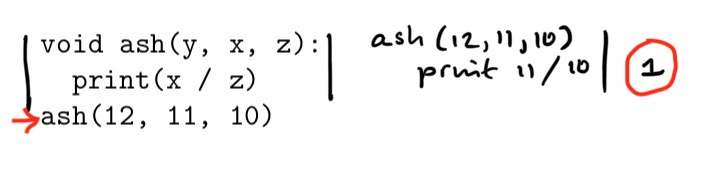
\includegraphics[width=.8\textwidth]{2-trace-params.jpeg}

Op de startregel staat een functieaanroep. Deze aanroep nemen we over rechts van de functiedefinitie. De functiedefinitie nemen we ook over, maar we vullen alle waarden zo \textbf{concreet} mogelijk in. De parameters \texttt{y}, \texttt{x} en \texttt{z} hebben in de concrete versie waarden gekregen, dus vullen we die ook in op de \texttt{print}-regel.

Tot slot blijft er nog een berekening over in het \texttt{print}-statement. Als we die evalueren, krijgen we het getal dat er geprint zal worden.

